\section{\CS: A Computational Fluid Dynamics code}
\label{sec:cs}
\CS is a computational fluid dynamics software designed to solve the
Navier-Stokes equations in the cases of 2D, 2D axisymmetric or 3D
flows. Development started in 1997, with a first release in 2000, and the
code has been released as free software under a GPL licence since 2007.
Its main module is designed for the simulation of flows which may be
steady or unsteady, laminar or turbulent, incompressible or potentially
dilatable, isothermal or not. Scalars and turbulent fluctuations of scalars can
be taken into account. The code includes specific modules, referred to as
``specific physics'', for the treatment of atmospheric flows, Lagrangian particle
tracking, semi-transparent radiative transfer, gas combustion, pulverised coal
combustion, electricity effects (Joule effect and electric arcs) and
compressible flows. \CS relies on a finite volume discretisation and
allows the use of various mesh types which may be hybrid (containing several
kinds of elements) and may have structural non-conformities (hanging nodes).The
parallelization is based on standard spatial partitioning with ghost cells
that facilitate data passing between adjacent cells lying across the boundaries
of disconnected parts using the Message Passing Interface. More
technical details are presented in~\cite{cs2004} and ~\cite{userguide},
and many resources are available at \url{http://www.code-saturne.org}.
\CS is also used as a base for the NEPTUNE\_CFD code, specialized in
multiphase flows, and which uses a different time stepping scheme,
but mostly the same volume discretization scheme.

As \CS is used for industrial cases involving complex flows, with turbulence
modeling requiring sufficiently fine resolution, large meshes are often
needed. In 2000, the largest meshes used for actual studies were around
1~500~000 cells; today, they have reached up to 350~000~000 million cells.
More common studies use meshes about 10 times smaller than that.
Meshes up to 3.2 billion cells have been tested for a few time steps, to
ensure the code's internal mechanisms work well at scale.

\CS focuses on the solver, and its uses requires external tools for the
major part of the meshing and visualisation tasks, though the code itself offers
major preprocessing features to make these easier, such as parallel joining
of independently-built and read submeshes (whether conforming or not),
and user-definable postprocessing functions. Many input mesh and visualisation
output formats are supported (including the EDF and CEA MED format,
and the standardized CGNS format).

~\
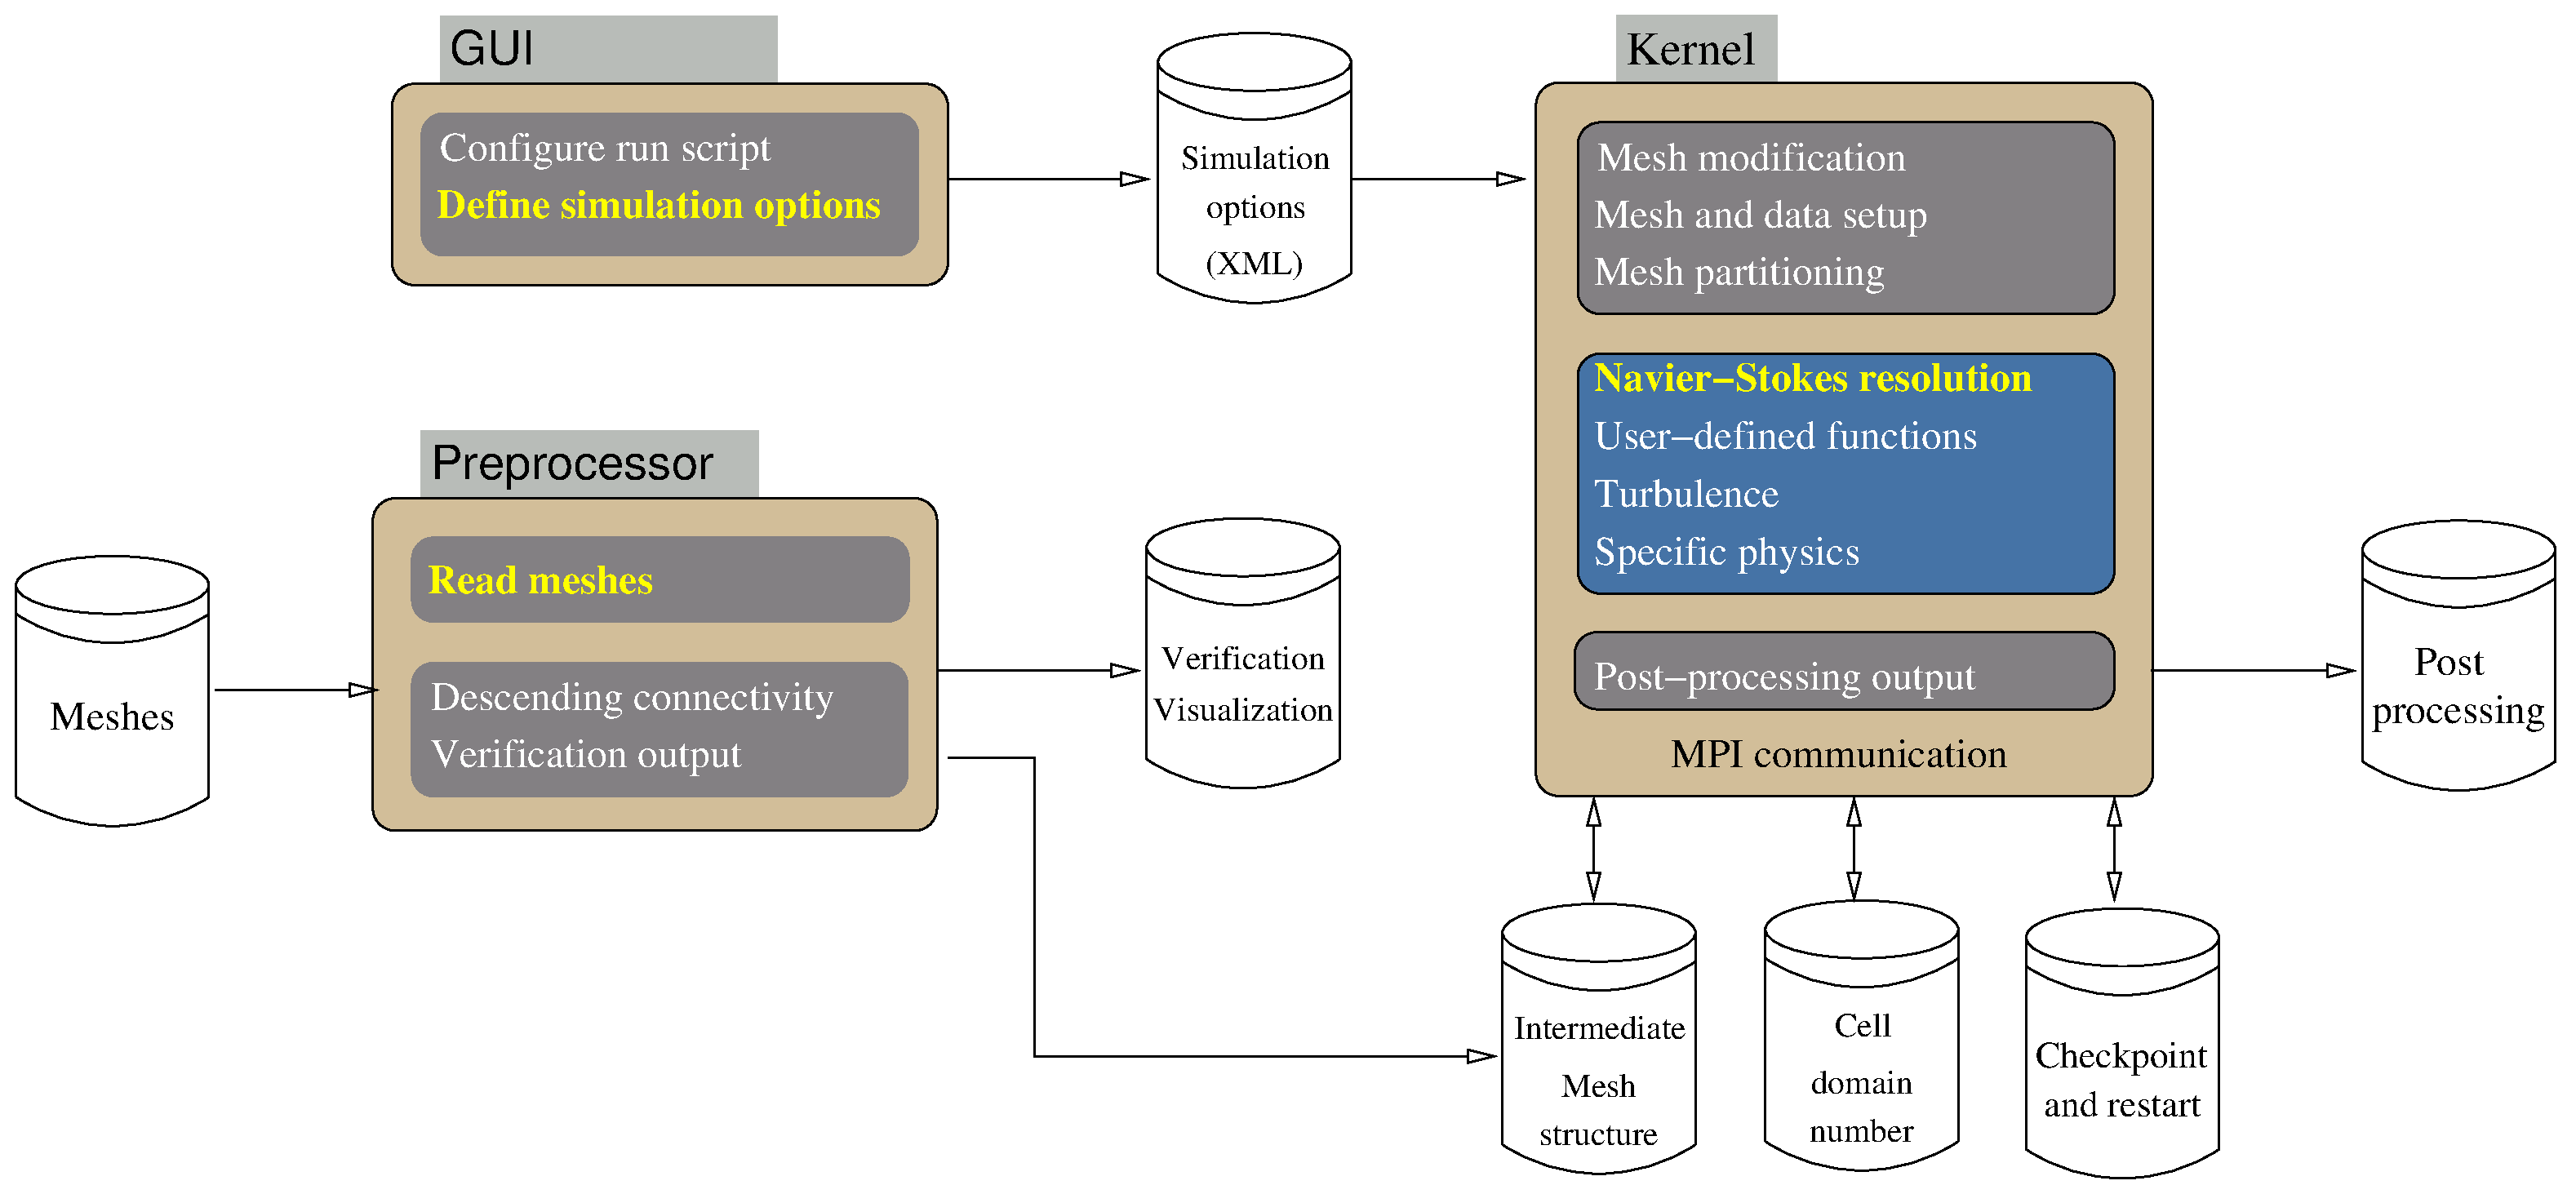
\includegraphics[scale=0.2]{pictures/cs_components.eps}
\captionof{figure}{\CS toolchain components.}
\label{fig:cs_components}
\vspace{+0.04in}
~\

The number of separate executable tools is quite reduced, with a few
interactive tools and associated commands designed for data setup,

To make it possible to work with large meshes and potientally long-running
simulations of unsteady flows, multiple postprocessing-related features
are available in the code. The user may specify 3D visualisation
output of selected main and auxiliary variables, time-plot data output
for selected cell values (``probes''), and 1-D profiles, as well as
choose to compute and log or output additional values by programming
a user function called at the end of each time step.
In this way, low-volume and global variables may be output
at each time step, and higher-volume output may be output with lower
frequency.

Mesh-based postprocessing output uses the concepts of \emph{meshes}
and \emph{writers}, as shown in the following figure:

~\
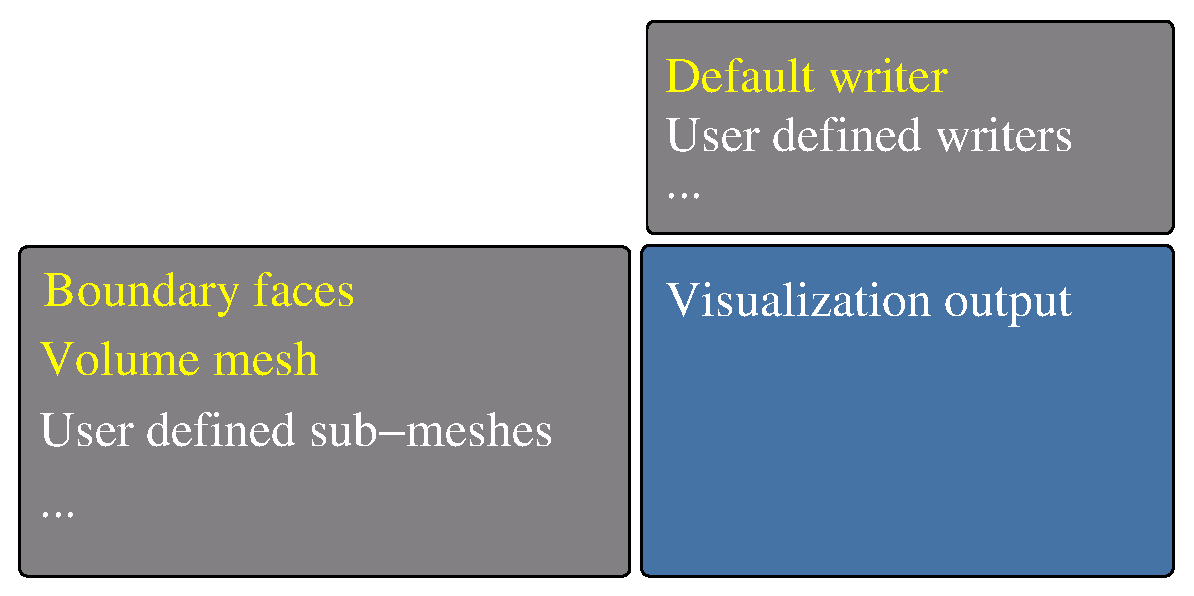
\includegraphics[scale=0.3]{pictures/cs_post.eps}
\captionof{figure}{\CS postprocessing output subsystem.}
\label{fig:cs_post}
\vspace{+0.04in}
~\

A mesh may be any sub-mesh of the computation mesh (or even
a separate auxiliary mesh in some cases), which may optionnaly
be redefined over time steps, while a writer is a combination of the
selection of an output format (such as EnSight gold, MED, or CGNS),
an output frequency, sub-directory and file name prefix,
and additional metadata specifying for example whether associated meshes
will be fixed or time varying (if the selected format supports it).
To each postprocessing \emph{mesh} may be associated a list of
\emph{writers} among those defined (an empty list meaning no output).
By default, the global volume mesh and boundary \emph{meshes} are
associated to a main \emph{writer}, whose default settings include the
EnSight gold format and output at the last time step only.
The user may modify those settings and associations, as well as
define additional \emph{meshes} and \emph{writers}, both using
the GUI and user functions (useful for more advanced cases
and finer control).
Using this system, output at different mesh formats, with different
frequencies, and possibly different variables may be generated
simultaneously, allowing fine tuning depending on the indended
usage.

\CS suggests a clear separation of tasks best handed by the code
or those handled by external tools. For example, although computing
a gradient may be handled directly by visualization tools, it is
best done in the user-defined output of the code itself, to ensure
it is done in a manner consistent with the discretization, and
exploiting the knowledge of prescribed boundary conditions.
On the other hand, postprocessing \emph{meshes} are defined as
subsets of the computational mesh, but generation of clips and slices
are not handled by the code, as it is expected visualization tools
may handled those geometric operations. Both may be combined: for example,
a volume sub-mesh involving cells around a clip plane may be output
by \CS, reducing the data that needs to be handled by a visualization
tool to produce that clip.
